\newthought{\textbf{Rauzatinur Syah - 2020903430039 - TRKJ 3B}}


\newday{\textbf{22 September 2022}}
\begin{enumerate}
\item Kendala dan Solusi\\
% jelaskan kendala dan penyebab yang dialami saat mengikuti praktikum serta solusi atau langkah-langkah yang telah dilakukan
kendala:
1. terdapat kendala pada instalasi hadoop pada pengecekanan versi hadoop yang berfungsi untuk menverifikasi instalasi hadoop\\
2. terdapat kendala saat menjalanakn format HDFS dan hadoop service

solusi:\\
1. melakukan pengecekan pada file hadoop-env.sh\\
2. melakuka  pengecekan pada file core-site.xml, hdfs-site.xml,mapred-site.xml, yarn-site.xml

\item Kesimpulan\\
% berikan kesimpulan dari praktikum yang telah dikerjkan
adapun kesimpulan yang diperoleh yaitu instalasi dan konfigurasi hadoop berhasil 

\end{enumerate}

\newday{\textbf{1 Desember 2022}}
\begin{enumerate}
\item Kendala dan Solusi\\
% jelaskan kendala dan penyebab yang dialami saat mengikuti praktikum serta solusi atau langkah-langkah yang telah dilakukan
pada pratikum Program WordCount bawaan hadoop tidak ada kendala pada praktikum yang dilakukan
\item Kesimpulan\\
% berikan kesimpulan dari praktikum yang telah dikerjkan
berhasil menjalanakan program wordCount bawan hadoop
\newpage
\begin{figure}[!ht]
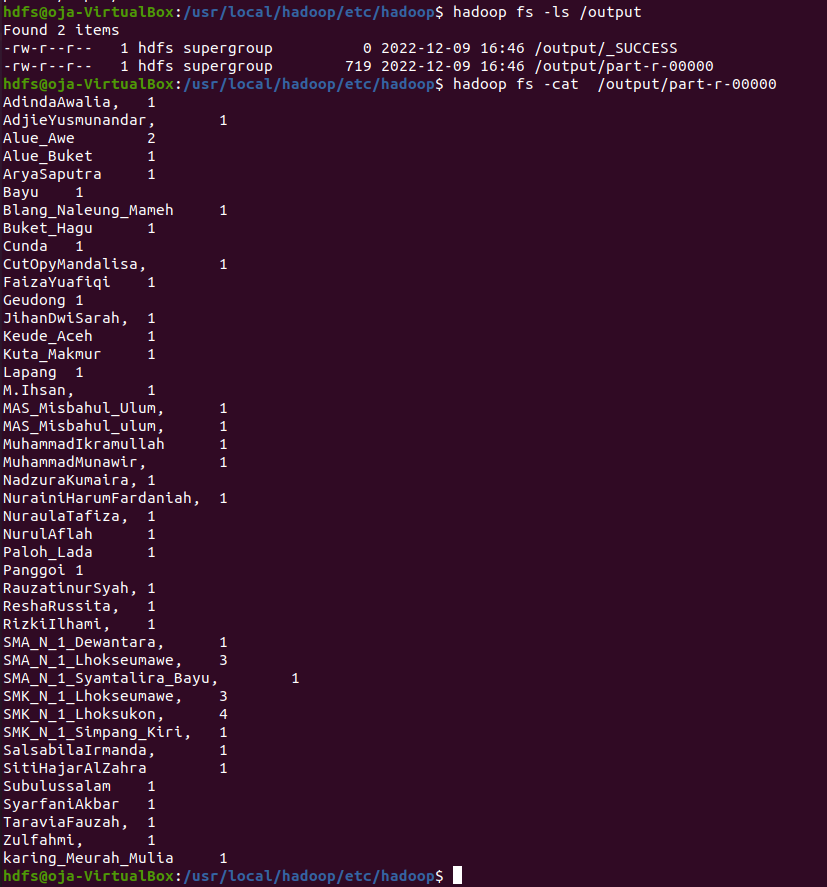
\includegraphics[width=\textwidth]{dataHadoop}
\caption{hasil program WordCount hadoop}
\label{gam:Hasil}
\end{figure}

\end{enumerate}


\newday{\textbf{2 Desember 2022}}
\begin{enumerate}
\item Kendala dan Solusi\\
% jelaskan kendala dan penyebab yang dialami saat mengikuti praktikum serta solusi atau langkah-langkah yang telah dilakukan
pada praktikum WordCount dengan java 
kendala:
terdapat kendala pada perintah menjalankan program dengan perintah"hadoop jar WordCount.jar WordCount /input/data/WordCount.txt /ResultWourdCountJava"
solusi:
menjalankan hadoop service dengan perintah "start-all.sh" dikarnakan terdapat kesalahan yang dilakukan yaitu tidak menjalankan hadoop service

\item Kesimpulan\\
% berikan kesimpulan dari praktikum yang telah dikerjkan
adapun kesimpulan yang diperoleh yaitu berhasil menjalankan programa tersebut 

\begin{figure}[!ht]
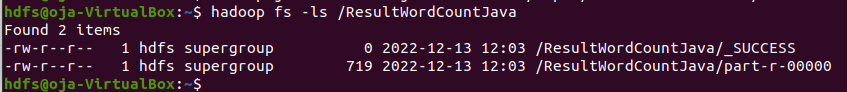
\includegraphics[width=\textwidth]{datahadoopjava no 9}
\caption{hasil program WordCount java no.9}
\label{gam:hasil program}
\end{figure}

\begin{figure}[!ht]
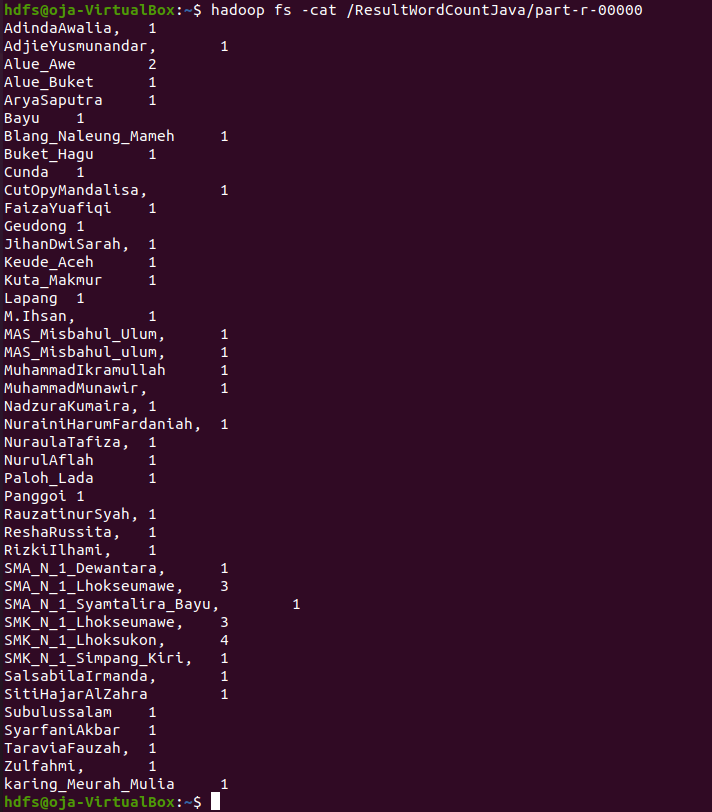
\includegraphics[width=\textwidth]{datahadoopjava no 10}
\caption{hasil program WordCount java no.10}
\label{gam:hasil program}
\end{figure}

\end{enumerate}

\newday{\textbf{08 Desember 2022}}
\begin{enumerate}
\item Kendala dan Solusi
% jelaskan kendala dan penyebab yang dialami saat mengikuti praktikum serta solusi atau langkah-langkah yang telah dilakukan

\item Kesimpulan
% berikan kesimpulan dari praktikum yang telah dikerjkan

\end{enumerate}

\newday{\textbf{09 Desember 2022}}
\begin{enumerate}
\item Kendala dan Solusi
% jelaskan kendala dan penyebab yang dialami saat mengikuti praktikum serta solusi atau langkah-langkah yang telah dilakukan

\item Kesimpulan
% berikan kesimpulan dari praktikum yang telah dikerjkan

\end{enumerate}